\chapter{Riemann Pump circuit design}
\label{ch:design}
% \textit{Description of the approach you have taken to solve the scientific or technical problem which you were posed. Outline the design, the methodology and overall structure of your experimental approach}\\
The aim of this thesis was to design an arbitrary waveform generator for a baseband signal bandwidth of \SI{6}{\giga \hertz}.
For the implementation in a base station, the most promising technology was \gls{ab:gan} \cite{EvertsDasKeybusJ.EtAl2010}, \cite{PengellyWoodMilliganEtAl2012}, \cite{SchmidReberChartierEtAl2011}.
\gls{ab:gan} \glspl{ab:hemt} were used for the high speed switches  \cite{MaroldtHauptKieferEtAl2009}, \cite{HongMukaiGheidiEtAl2013}, \cite{MaroldtBruecknerQuayEtAl2014}, \cite{WentzelMelianiHeinrich2010}, \cite{MaroldtQuayHauptEtAl2011}, \cite{QuayMaroldt2011}, which served as voltage controlled current sources, in this concept.
Based on the chosen technology, a suitable push-pull concept were found \cite{MaksimovicPaper} to show the feasibility of the concept.
The attention was rather drawn to prove the concept than to optimize for energy consumption or efficiency.
In the design process, a suitable load impedance and the right dimension of the used components had to be found.

\section{Approach and implementation of the Riemann Pump}
As stated in chapter \ref{IdeaRiemannPump}, the circuit needed high speed switches, which were capable to drive power.
In order to switch a \gls{ab:hemt} transistor to the high side power rail, a driver circuit was needed, since in \gls{ab:gan} technology no complementary transistors were available.
The absence of a p-type transistor made it challenging to find a suitable concept to realize the push-pull stage.
The n-type \glspl{ab:hemt} operating in depletion mode, needed a negative gate source voltage \gls{sy:vgs} to switch the transistor off.
For the on switching, \gls{sy:vgs} had to be \SI{0}{\volt} and therefore a driver circuit was needed \cite{Y.Zhang2015}, \cite{MaksimovicPaper}, \cite{GhoshAltmannKerstenEtAl2014}, \cite{HongMukaiGheidiEtAl2013}, since the source potential of the high side switch varies between \gls{sy:Vdd} and \gls{sy:Vss}.
The source contact of the high side switch, realized by a n-type \gls{ab:gan} \gls{ab:hemt}, was connected to the output of the test circuit and therefore the potential at the output was not constant.
A suitable driver circuit was found in \cite{MaksimovicPaper}, where the principle of a push-pull stage for power applications is described.\\
One possible approach to design a Riemann Pump is shown in Fig. \ref{fig:SchematicRiemannPump}.

\begin{figure}[ht]
	\centering
  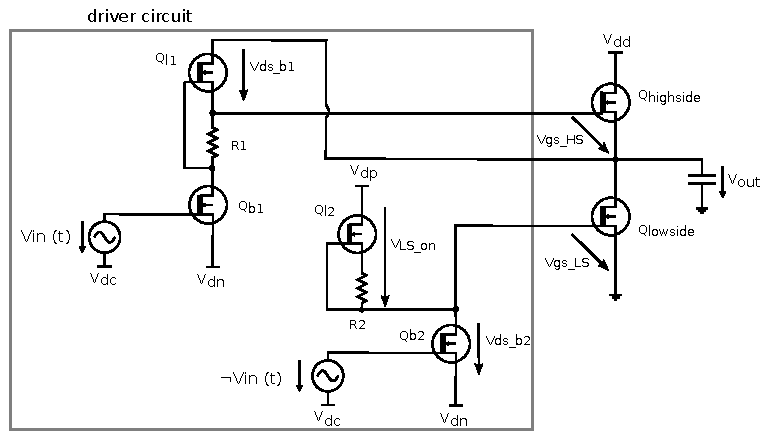
\includegraphics[width=\textwidth]{Schematic_RP_concept2.pdf}
	\caption{Schematic of a push-pull stage with corresponding driver circuit}
	\label{fig:SchematicRiemannPump}
\end{figure}

%%%%%%%%%%%%%%% 00:40 Uhr 01.05.2016
On the left side, as marked, the driver circuit is depicted which was needed to switch the high side transistor without dissipating a huge amount of power.
As the timing is crucial for the switching process, the driver concept was implemented for the low side switch too.
Each driver consisted of a base transistor, marked as $Qb1$ and $Qb2$, which served to operate as an inverter.
Also two load transistors, $Ql1$ and $Ql2$, were implemented with a source degeneration resistor which served as a current source.
The resistors $R1$ and $R2$ were tuned to provide a proper current while maintaining a decent power consumption.
If the resistors were set to a low value, the current source provides more current and hence the switching process is faster, since the charging of the gate capacitance of the high and low side transistors is faster.
But a draw back was that for the higher current a higher power consumption occurred.
In addition to the driver circuit, two power transistors were implemented, which represented the one bit \gls{ab:dac}.
These two transistors, $Q_{highside}$ and $Q_{lowside}$, worked as switches which switch the output to the high side power rail and low side power rail, respectively.
Switching the high side transistor $Q_{highside}$ to the on state required a gate-source voltage $V_{gs\_HS}$ of \SI{0}{\volt}.
This is achieved by the feedback path from the output to the drain of the load transistor $Q_{l1}$ which also turns on and in fact of the low on resistance the voltage drop of $Vds\_b1 \approx 0 V$ ($\equiv V_{gs\_HS}$).
The transistor $Ql1$ is turned on because $Vgs\_b1 = 0 V$, since the base transistor $Qb1$ is turned off and hence no current is flowing.
Switching from the on to the off state happened, when the base transistor $Qb1$ is switched on with a control voltage.
When the base transistor is turned on, the gate potential of the high side transistor is set to approximately \gls{sy:vdn}, by discharging the gate capacitance with $Ql1$ and $R1$ which served as a current source.
The dimension of $Ql1$ and $R1$ determined the discharge current for $Q_{highside}$ and hence the switching speed and the power losses.
Because $Q_{highside}$ is turned on if $Qb1$ is turned off and inversely, this act as a inverter structure.
In addition to the presented principle of the high side switch, the low side circuit operated in the same way but inversely.
When the high side switch is turned on, the low side is turned off and vice versa.
The benefit of the integrated driver circuit was the improved efficiency of switching.
The transistor switching speed was determined by the dimension of the driver circuit.
The schematic shows the first approach for realizing a Riemann Pump in \gls{ab:gan} technology.
The next step was the identification and calculation of a proper output capacitance, since it represented the input of a linear power amplifier, where the desired signal is synthesized.
 
 %% 09.05.2016 01:33 Uhr
\section{Identification of the load impedance} % VERBESSERN!
Due to the fact that the signal is generated at the input stage of a linear power amplifier, as described in chapter \ref{ch:fundamentals}, it was crucial to obtain its input impedance.
The input impedance of the power amplifier was at the same moment the output impedance for the test circuit. 
This output stage of the test circuit is modelled with a \gls{ab:gan} \gls{ab:hemt} with a gate length of \SI{0.25}{\micro \meter}.
Considering a \SI{20}{\watt} power amplifier for transmission purposes, led to a \gls{ab:gan} \gls{ab:hemt} with a total gate periphery of \SI{4}{\milli \metre}, based on an approximation for the power density of \SI[per-mode=fraction]{5}{\watt\per\milli\metre} gate periphery  \cite{Maroldt2010}, \cite{GaNBook}.
Simulations confirmed this approximation as an output power density of \SI[per-mode=fraction]{5.6}{\watt\per\milli\metre} at $V_{GS} = -1.5 V$, $V_{DS} = 25 V$ was measured.
The transistor model used in \gls{ab:ads} were modelled at the \gls{ab:iaf} \cite{Model} and is based on a state-space approach. 
For simulation purposes four transistors were modelled in parallel, each with 8 finger and \SI{125}{\micro \metre} gate width to reach the required gate periphery.
The simulated power amplifier is biased with respect to the maximum \gls{ab:mag} \cite{DeltimpleLeyssenneKerherveEtAl2010}, which led to a bias of $V_{GS} = -1.5 V$ at $V_{DS} = 25 V$.
After the determination of the bias point, a S-parameter simulation yielded the input reactance of the power amplifier.
It is to note that the short analysis of the impedance was done with four power transistors in parallel representative for a power amplifier than a discrete model of a broadband amplifier.
But since it was not the main goal to obtain a proper input impedance of a broadband amplifier this identification was sufficient.
Hence this was a short and effective way to obtain an output impedance according to the equivalent circuit of a \gls{ab:hemt} device as shown in Figure \ref{fig:eqcircuit}.

\begin{figure}[H] % small signal equivalent circuit
	\centering
  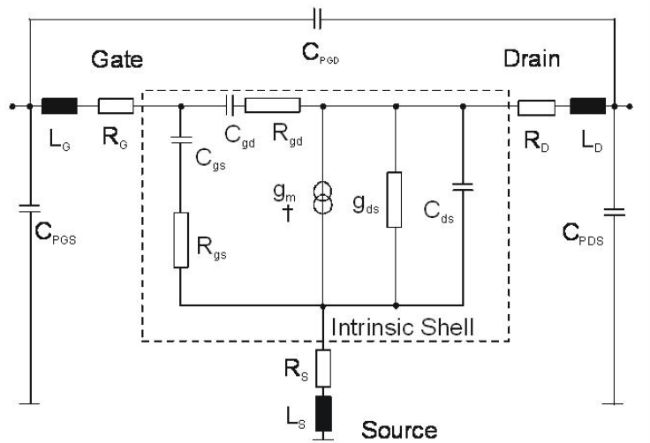
\includegraphics{equivalentcircuit_hemt.pdf}
	\caption{\gls{ab:rf} equivalent circuit \gls{ab:fet} \cite{Quay2014}}
	\label{fig:eqcircuit}
\end{figure}

The input of the \gls{ab:hemt} is determined by the capacitances $C_{gs}$ and $C_{gd}$, since the inductance is effective only for high frequencies \cite{LSModel}.
This capacitive behaviour is seen in Figure \ref{fig:eqcircuit} for the gate node, which served as the input.
As only the capacitive behaviour of the load impedance was of interest, the real part was neglected.
The complex impedance is defined as
\begin{equation}
	Z = R + jX,
\label{eq:impedance}
\end{equation}
where R is the real part and X is the electrical reactance.
%The capacitive reactance $X_c$ is defined as:
The electrical reactance $X$ is defined as:
\begin{equation}
	X = X_{L} + X_{C} = \omega L -\frac{1}{\omega C},
\label{eq:reactance}
\end{equation}

and is plotted for the input of the test power amplifier in Figure \ref{fig:inputReactance} over the frequency range from nearly \gls{ab:dc} to \SI{6}{\giga \hertz} in a logarithmic scale.

\begin{figure}[H]
	\centering
  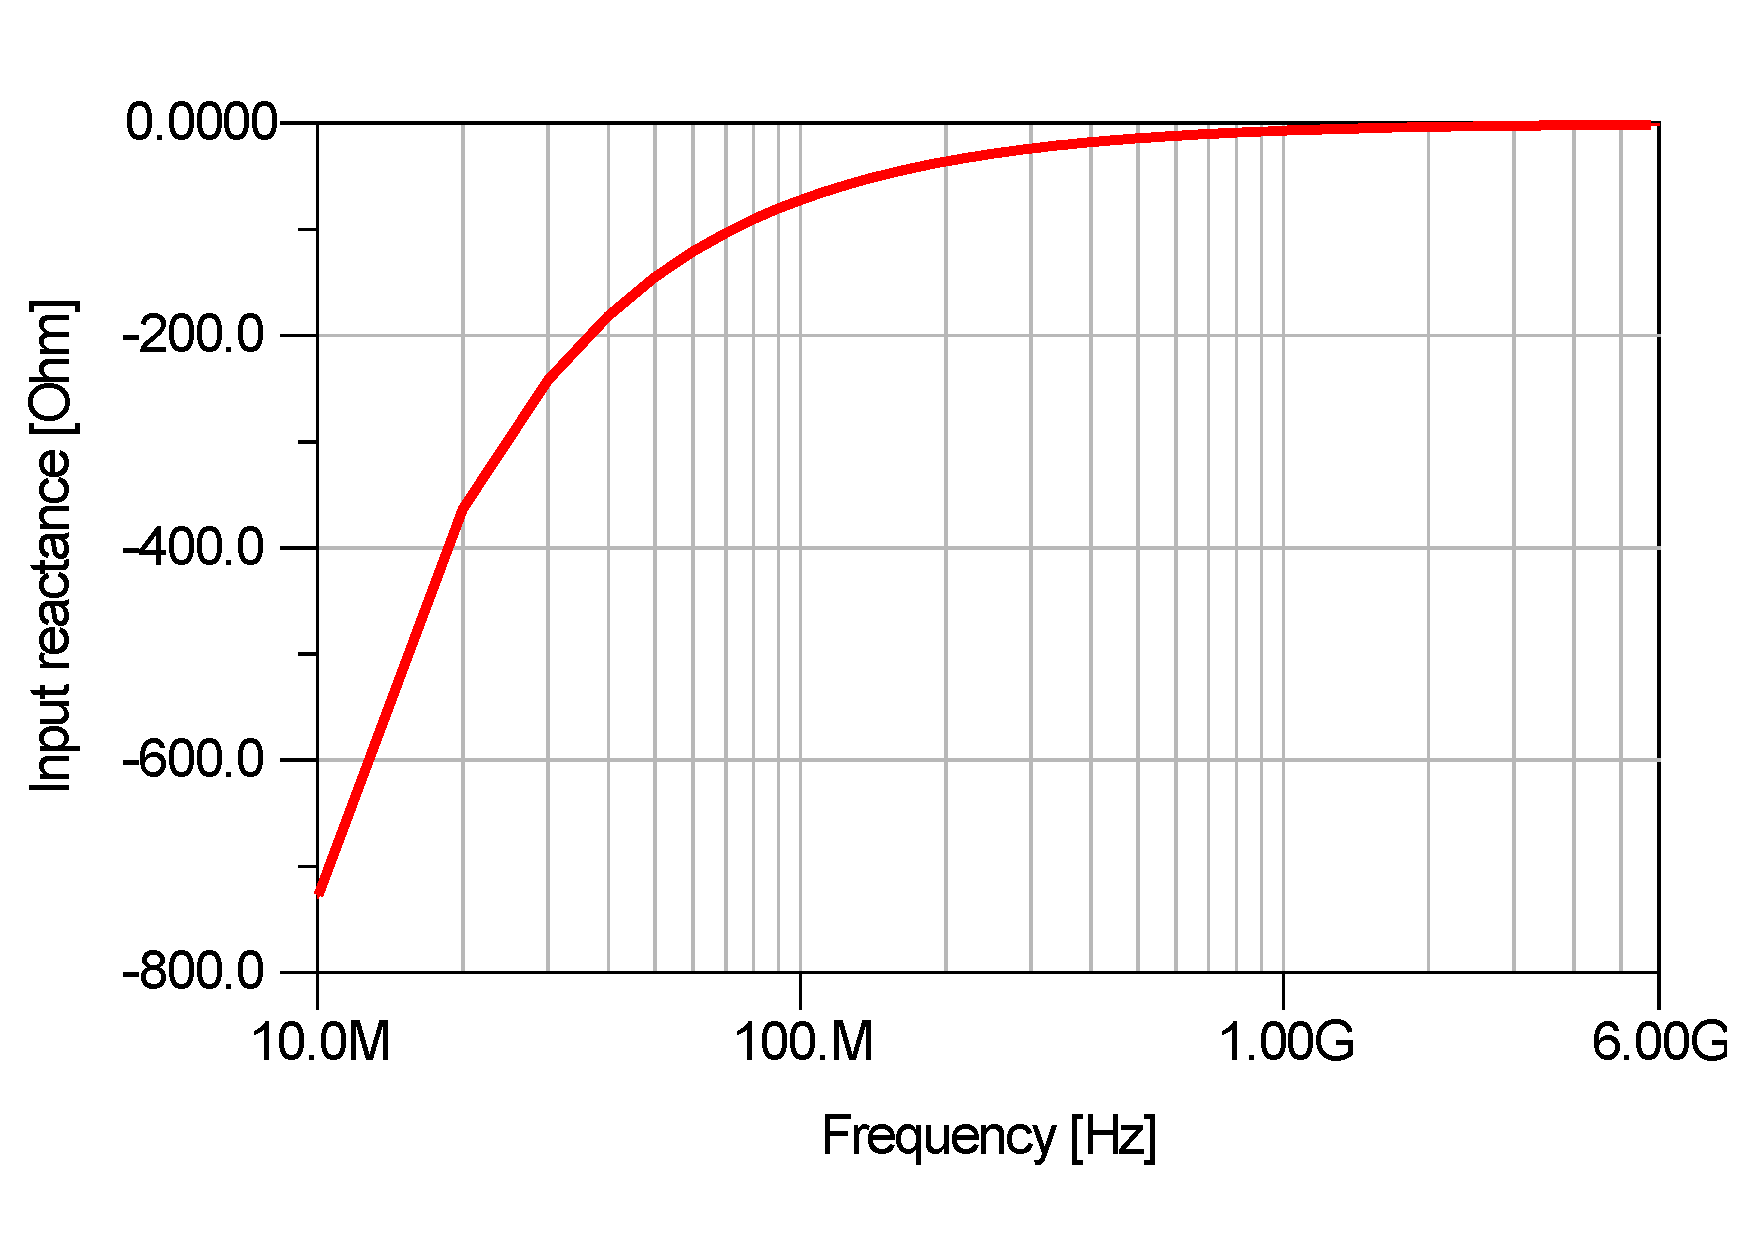
\includegraphics[width=.75\textwidth]{inputReactance.pdf}
	\caption{Load reactance over frequency in logarithmic scale}
	\label{fig:inputReactance}
\end{figure}


The constant increase of the reactance to nearly \SI{0}{\ohm} confirmed Equation \ref{eq:reactance}, since the main part of the reactance is determined by $X_{C}$.
The capacitive reactance $X_{C}$ is defined as:

\begin{equation}
	X_{C} = -\frac{1}{\omega C},
\end{equation}

and thus the reactance scales with the reciprocal value of $\omega$.
The input capacitance $C_{in}$ determined by the sum $C_{gs} + C_{gd}$, was calculated and yielded $C_{in}\approx 20 pF$.
This estimation of the input reactance was sufficient and parasitic effects were neglected \cite{CakaZabelliLimaniEtAl2007}, \cite{ZhangZhangTangEtAl2014}.
Consequently this capacitance is used for further investigation as a load impedance.
%Considering the absolute value of the reactance its value is decreasing.
%For frequencies beyond \SI{1}{\giga \hertz} the impact of parasitic inductances induced a constant value for the reactance.
%Interpreting the minus sign only for the phase delay, since it is capacitive, the absolute value of the reactance decreases exponentially with the frequency up to approximately \SI{1}{\giga \hertz}.
%Solving the equation \ref{eq:reactance} for the capacitance yielded:
%
%
%with respect to the absolute value of $X_c$.
%Figure \ref{fig:inputCap_log} illustrates the absolute value of $C_{in}$ and states the effect of the parasitic inductances.
%For low frequencies the parasitic inductances could be neglected, but for high frequencies these parasitic inductances effects the absolute value of the electrical reactance.
%Therefore it seemed that the capacitance is decreasing for frequencies in the \si{\giga \hertz} range.
%
%%The frequency dispersion effect on the input capacitance of the \gls{ab:gan} \gls{ab:hemt}
%\begin{figure}[H]
%	\centering
%  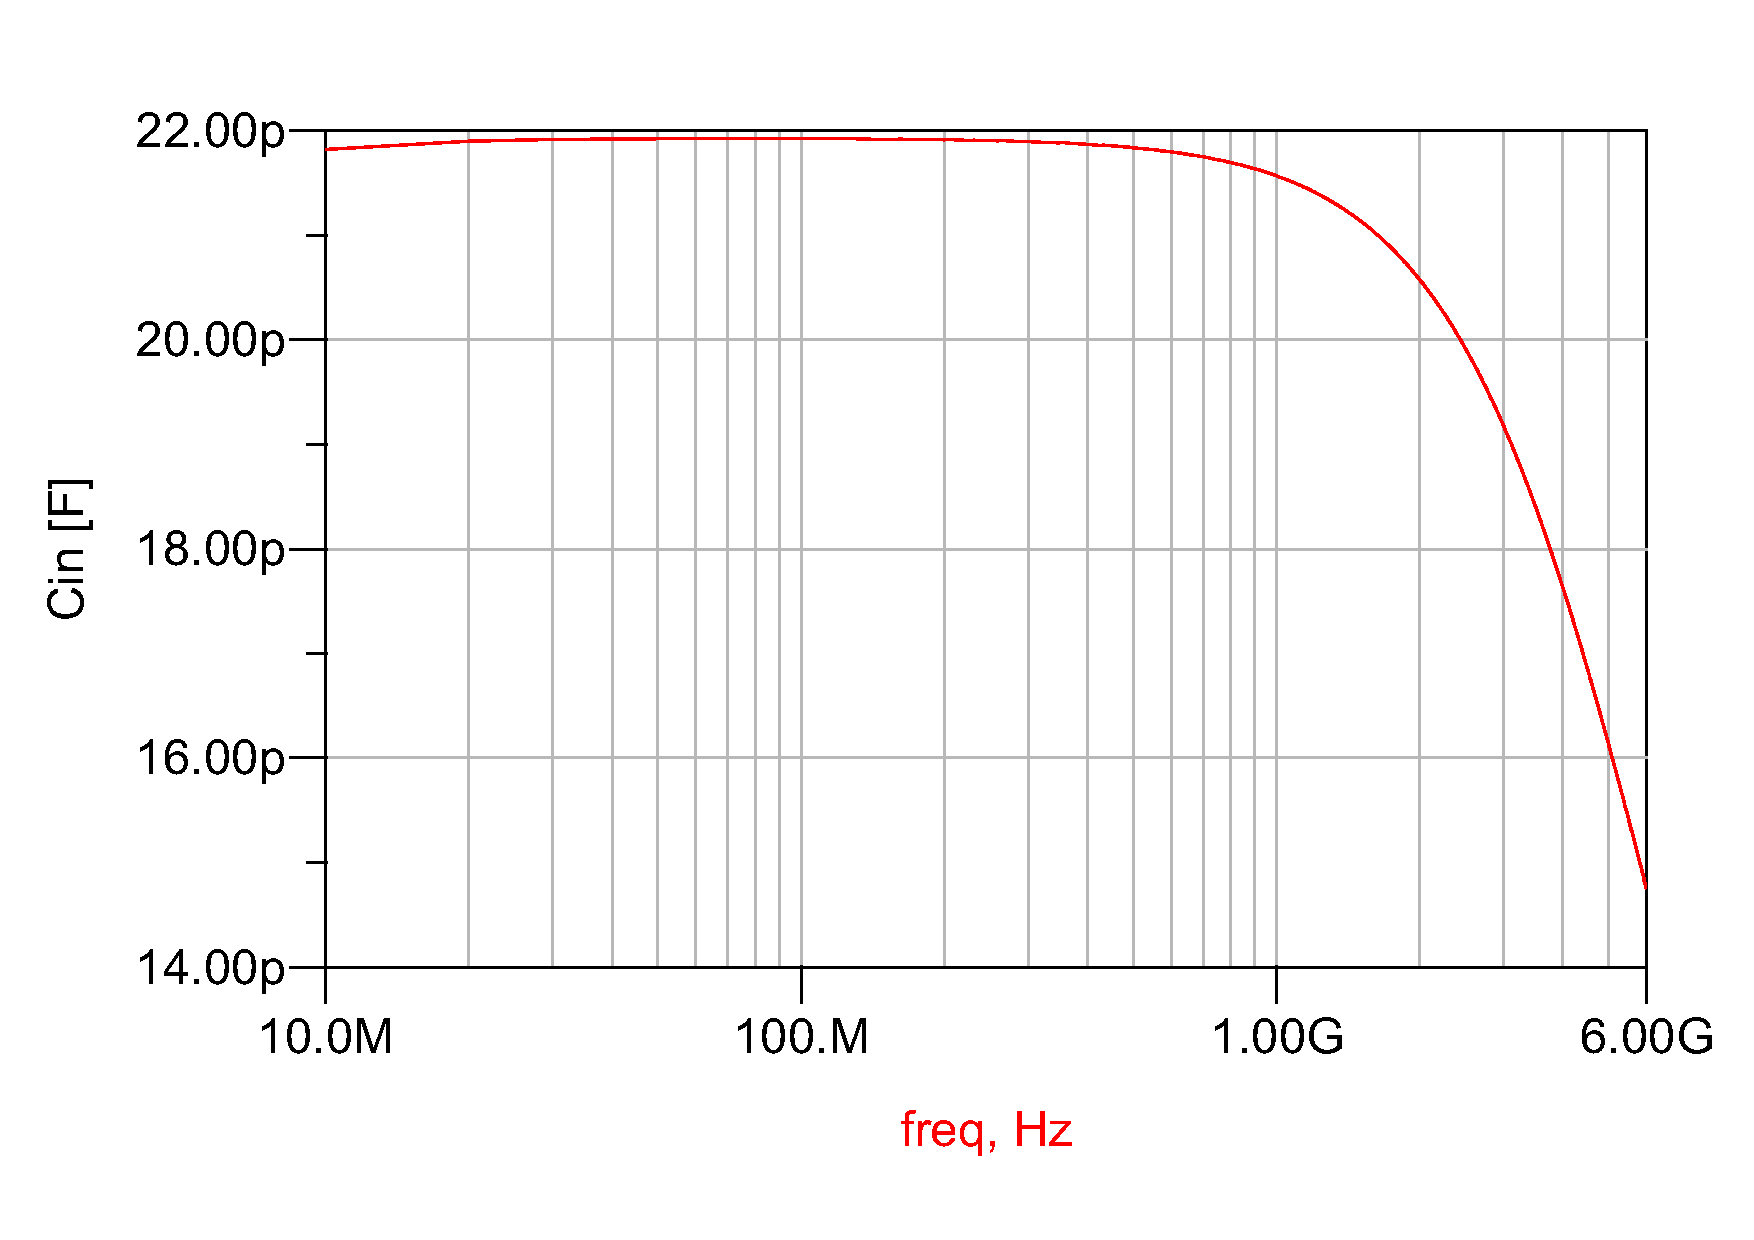
\includegraphics[width=.75\textwidth]{inputCap_log.pdf}
%	\caption{Load capacitance over frequency in logarithmic scale}
%	\label{fig:inputCap_log}
%\end{figure}

%Nevertheless the complex input impedance yielded a capacitive behaviour with a value of nearly \SI{22}{\pico \farad}, which was used for further investigations.
%The simulated transistor model was specified as a large signal model
% small signal is not considered, since only the curent integration is important

%%% 27.04.2016 01:34 Uhr
\section{Dimension of the used components}
An input capacitance of nearly \SI{20}{\pico \farad} was found for the output linear power amplifier stage.
Based on this calculation a proper test circuit was investigated.
To avoid immediate clipping of the signal at the output, the transistor dimension had to fit, since an oversized transistor would fully charge the capacitance and the signal would be clipped.
Hence a transistor dimension was chosen which allowed to synthesize a decent signal.
To synthesize a sine wave for the frequency of \SI{6}{\giga \hertz} with a voltage swing of $V_{swing} = 4V$, the two greatest slopes were chosen.
In the presented concept the resolution is three bit, hence eight different current slopes could be generated.
The sequence of the relative slopes $7 i_0$ and $5 i_0$ synthesize the rising edge of the sine wave.
With this relative slopes and an oversampling ratio of four at the frequency of \SI{6}{\giga \hertz}, led to a sampling time $\Delta t$ of \SI{20.83}{\pico \second}, since the sampling frequency is eight times the signal bandwidth.

The current-voltage relation for the capacitor
\begin{equation}
	I = C \frac{d U}{d t},
\end{equation}
is used to determine the reference current $i_0$.

A voltage swing of $V_{swing} = 4V$ is equal to an amplitude of $\hat{v} = 2V$.
The oversampling of four yielded, that the sine signal is sampled by eight points.
Hence the rising edge consisted of two sampling points.
The first sampling point with the relative slope of 7 and the second of 5, respectively.
Integrating the current for two different samples yield:

\begin{equation}
\int_{\Delta t} 7 i_0 d\tau + \int_{\Delta t} 5 i_0 d \tau = C*U,
\end{equation}

and solving for $i_0$ resulted in:

\begin{equation}
i_0 = \frac{U*C}{12*\Delta t}.
\end{equation}

For the assumption to reach nearly a voltage of $U = 2V$ for two sampling intervals ($2 \Delta t$) and the capacitance of \SI{20}{\pico \farad} it resulted a reference current of $i_0 = \SI{160}{\milli \ampere}$.
%The dimension of the switching transistors, which represent a voltage controlled current source, determines the maximum current flowing.
%This current source is controlled by a digital signal which determines it to be fully open or to be closed, as a switch.
As simulations showed, a reference current of $\SI{151}{\milli \ampere}$ could be established with a dimension of the voltage controlled current source, high side switch, of UGW = 100 \si{\micro \meter} and gate finger number of eight.
Hence the gate periphery for the reference current source is \SI{800}{\micro \meter}.
To ensure proper switching the driver circuit dimension had to be optimized.
Since the driver circuit worked as a current source, the dimension of the transistors and resistors were tuned to achieve a proper current to switch the power transistors fast and efficient.
The dimension of the driver transistors were approximately a quarter of the power transistors, the switching high and low side transistor.
The resistor values were achieved by tuning with respect to power consumption.
Further details on the driver circuit and its properties are stated in \cite{MaksimovicPaper}.
Figure \ref{fig:RealCircOne} demonstrates one bit of the realized circuit.

\begin{figure}[H]
	\centering
  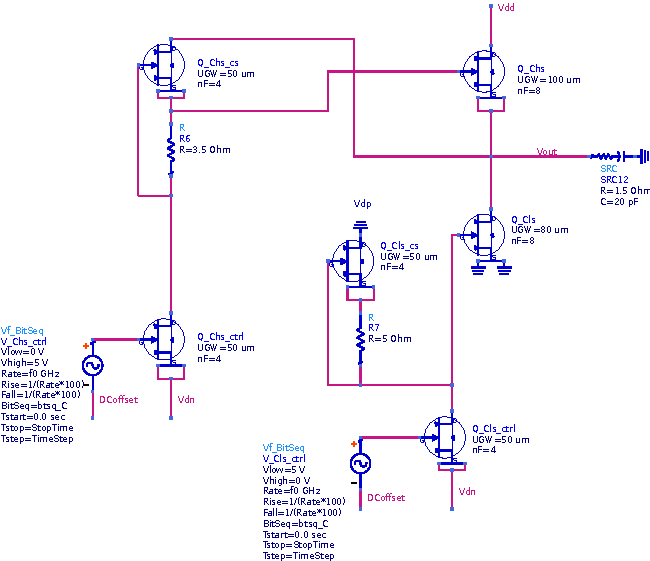
\includegraphics{realizedCircuit_oneBit.pdf}
	\caption{One bit of the realized circuit}
	\label{fig:RealCircOne}
\end{figure}

The schematic is designed with \gls{ab:ads} and the full circuit design can be seen in Appendix \ref{app:schematic}.
For the full schematic it is to note that the dimension of the power transistors scales with the factor of two and so the driver circuit dimension do.

\section{Identified problems}
During the design process some problems already occurred.
The major problem was that the current sources could not be defined as necessary.
One requirement to use a \gls{ab:gan} \gls{ab:hemt} as a voltage controlled current source is depicted in Figure \ref{fig:OutputCharacteristic}.
In this simulation an unloaded transistor with eight gate fingers and a gate unity width of \SI{125}{\micro \meter} was used.

\begin{figure}[ht]
	\centering
  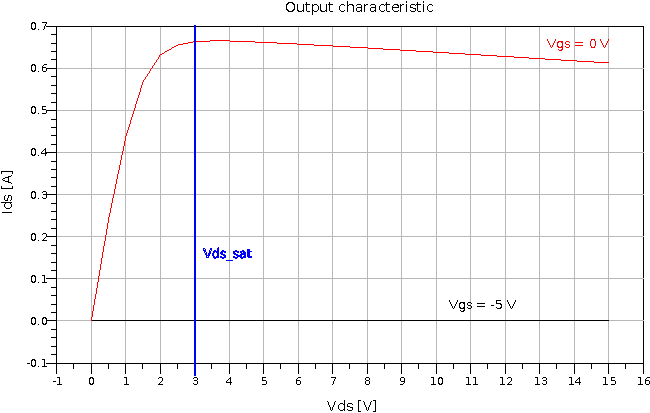
\includegraphics{outputCharacteristic.pdf}
	\caption{Output characteristic of a \gls{ab:gan} \gls{ab:hemt} in depletion mode}
	\label{fig:OutputCharacteristic}
\end{figure}

Figure \ref{fig:OutputCharacteristic} shows the output characteristic of a \gls{ab:gan} \gls{ab:hemt} in depletion mode for $V_{gs}$ of \SI{0}{\volt} (red) and \SI{-5}{\volt} (black).
The blue line marks the transition from the linear to the saturation region.
The on state is marked red with a gate-source voltage of \SI{0}{\volt}.
If the transistor is switched off no current is flowing, refer to the black curve with gate-source voltage of \SI{-5}{\volt}.
To ensure that the \gls{ab:gan} \gls{ab:hemt} in depletion mode acts as a voltage controlled current source, it is necessary that $V_{gs} = 0V$ and $V_{ds} \geq V_{ds,sat}$.
Hence the transistor had to be in the saturation region.
The simulation yielded a drain-source saturation voltage of approximately \SI{3}{\volt}.
For the linear region, $V_{ds} < V_{ds,sat}$, the transistor acts as a resistor than a defined current source.
This condition made it difficult to generate a reference current.
Therefore a requirement would be, that the output voltage only vary between $V_{ss} + V_{ds,sat}$ and $V_{dd} - V_{ds,sat}$.
Once this limit is reached the current is not defined any more.
As simulation showed, this problem occurred for both the high and the low side switching transistor and can be seen that the relative slopes do not scale with the presented slopes.
In addition to this non ideal switching occurs which made it necessary to average the current over time.
The problem of not perfect switching is, that the channel is opened and closed slowly in comparison to an ideal switch and hence the current do not switch from zero to $i_0$ rather slowly increase.
A leakage current over the driver circuit is observed which further increase the problem.
It is to mention that every push-pull stage had to handle this problem and therefore the relative slopes are considered, but the stages differed in the behaviour of switching and hence $3 i_0$ is not perfectly $3 * 1 i_0$.
The different behaviour for the switching process of the separate push-pull stages led to a not precisely set of slopes. 
Reason for this was the leakage current of the driver network for the discharging process of each bit.


\section{Circuit design summary}
As no complementary transistors were available in III-V technology, a proper driver circuit had to be investigated.
Further the speed of the switches was crucial as a broadband signal should be synthesized, which led to the implementation of a known concept \cite{MaksimovicPaper} for the driver circuit.
A low loss, high speed, digital controlled driver circuit was implemented which had the advantage to be verified and validated.
The circuit design and simulation combines the \gls{ab:dc} state with the \gls{ab:rf} state, since for a \gls{ab:dc} simulation the current through a capacitor is zero.
The dimension of the used components with the sampling interval determined the resulting voltage step.
A draw-back was that a small transistor dimension could synthesize signals to a very low signal frequency while a bigger one would fully charge the output capacitor which will clip the output signal.
If the transistor dimension is chosen to be bigger, the higher signal frequency could be synthesized with a decent voltage swing but the low signal frequencies would turn into a rectangular shape. 
Therefore the dimension of the used components already limit the bandwidth.
The signal bandwidth was investigated to be smaller than \gls{ab:dc} to \SI{6}{\GHz}.
The used components were tuned with respect to the signal integrity over the frequency range of nearly \SI{1.5}{\giga \hertz} to \SI{6}{\giga \hertz}. 
%realized with multi chip assembling on a hybrid board.
%The smallest current is determined by the dimension of the transistor, which drives into saturation. 
%The smallest saturated current is determined by the push-pull transistor geometry, here: 532 mA.}